\documentclass{thesis}
\usepackage{bm,listings,jvlisting,ascmac,framed,color}
\usepackage{fancybox}
\lstset{%
	captionpos=b,
    basicstyle={\ttfamily\small}, %書体の指定
frame=tb, %フレームの指定
framesep=10pt, %フレームと中身(コード)の間隔
breaklines=true, %行が長くなった場合の改行
%linewidth=15cm, %フレームの横幅
lineskip=-0.1ex, %行間の調整
tabsize=3, %Tabを何文字幅にするかの指定
  numbers=left,%
    stepnumber=1,
  numbersep=1zw%
}


\makeatletter
\AtBeginDocument{%
	\let\c@figure\c@lstlisting
	\let\thefigure\thelstlisting
	\let\ftype@lstlisting\ftype@figure
}
\makeatother

\renewcommand{\lstlistingname}{図}
\begin{document}

% 目次
\tableofcontents

\chapter{序論}

高品質なソフトウェアを効率的に開発していく上で,....が重要である\cite{ソフトウェア工学の基礎知識}.
そこで本論文では....を行う.

本論文の構成は以下の通りである.
まず,第 \ref{chap:メトリクス} 章でソフトウェアメトリクスについて概説し,
第 \ref{chap:提案法} 章で○○に基づいた△△を提案する.
そして,第 \ref{chap:実験} 章でオープンソースソフトウェアを対象とした
評価実験を行い,提案法の有効性について考察する.
最後に第 \ref{chap:結論} 章で本論文のまとめと今後の課題について述べる.

\chapter{ソフトウェアメトリクス}
\label{chap:メトリクス}

\section{緒言}

本章では本論文での議論の準備として
ソフトウェアメトリクスについて概説する.
以下,\ref{sec:ソフトウェアメトリクスとは} 節でソフトウェアメトリクスの
定義とその大まかな分類を示す.


\section{Word2Vec}
Word2Vec\cite{word2vec}とは,学習の際にテキストデータを解析し,単語の意味を考慮して各単語をベクトル化する手法である.
これにより,単語同士の意味の類似度を計算したり,意味を足したり引いたりすることが可能になる.
Word2Vecの学習方法として,Continuous Bag-of-Words とSkip-gramが挙げられる.
Word2Vecはどちらかの方法に従い,ニューラルネットワークを用いて学習を行うことにより,単語をベクトル化する.
それぞれの学習方法の概要を以下に示す.
\begin{itemize}
	\item Continuous Bag-of-Words
	
	Continuous Bag-of-Words(CBoW)\cite{word2vec}は,周辺の単語から注目する単語を予測できるように学習を行う.
	例えば,``I have a cat at home''という文章の``cat''に着目して``I have a ○○ at home''という文章を考える.
	CBoWでは,この○○にどういった単語が入るかを予測するという考え方の下で学習を行う.
	○○に入る可能性のある単語を考えると,``cat''以外にも``dog''や``hamster''などが挙げられる.
	CBoWは,周辺の単語である``I'',``have'',``a'',``at'',``home''から○○に入る単語が``cat''だと予測できるように学習する.
	\item Skip-gram
	
	Skip-gram\cite{word2vec}は,注目している単語から周辺の単語を予測できるように学習を行う.
	先ほどの文章を例に挙げると,``cat''という単語からその前後に登場する単語``have''や``home''などを予測できるように学習する.
\end{itemize}

実際に``I have a cat at home''という文章に対してSkip-gramによる学習の流れを概説する.
まず,文字列の状態では計算することができないため,文字列をベクトル化するためにone-hotベクトルを考える.
one-hotベクトルとは,文字列中の単語の種類数に等しい次元のベクトルを考え,その単語に該当する要素を1,その他を全て0とするベクトルである.
例えば,各単語のone-hotベクトルは以下に示すベクトルとなる.

\begin{itemize}
	\item I : (1,0,0,0,0,0)
	\item have : (0,1,0,0,0,0)
	\item a : (0,0,1,0,0,0)
	\item cat : (0,0,0,1,0,0)
	\item at : (0,0,0,0,1,0)
	\item home : (0,0,0,0,0,1)
\end{itemize}

このとき,入力が``cat''のときのニューラルネットワークによる学習のイメージを図 \ref{fig:イメージ図} に示す.
ここでは隠れ層のユニット数を3としている.
隠れ層とは,データが入力される入力層と,結果を出力する出力層の間の層である.

\begin{figure}[H]
	\centering
	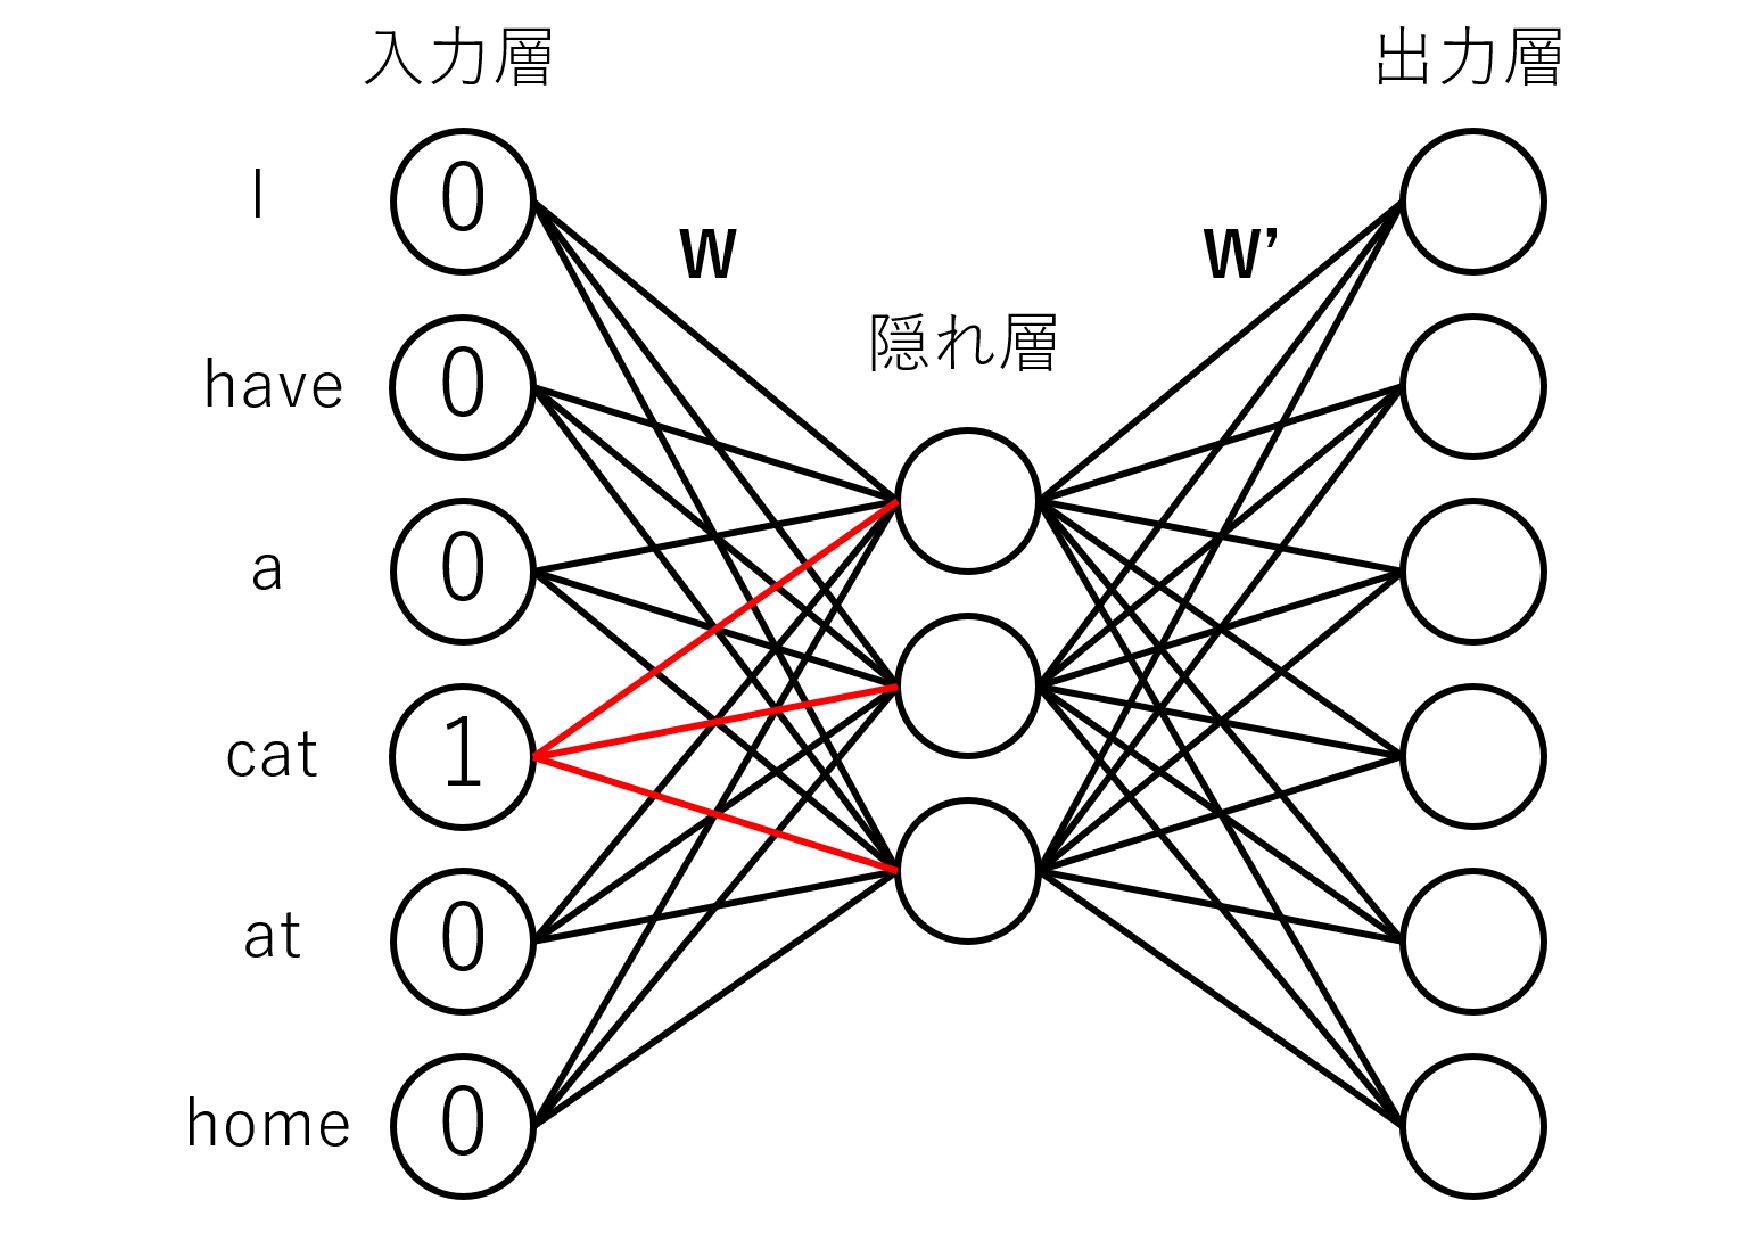
\includegraphics[scale=0.5]{./image/word2vec_nn.pdf}
	\caption{学習のイメージ図}
	\label{fig:イメージ図}
\end{figure}

次に入力層から隠れ層,隠れ層から出力層への重み行列を導入する.
ここで入力層から隠れ層への重み行列を\textbf{W},隠れ層から出力層への重み行列を\textbf{W'}とする.
また,隠れ層のユニット数は3としているため,重み行列の次元数は3である.
初期状態では,重み行列の内容はランダムに生成される.(\ref{eq:w})式のような重み行列\textbf{W}を考える.


\begin{align}
	\label{eq:w}
	\bm{W}=\left[
	\begin{array}{ccc}
		0.1 & 0.2 & 0.5 \\
		0.2 & 0.8 & 0.4 \\
		0.3 & 0.5 & 0.7 \\
		0.4 & 0.4 & 0.6 \\
		0.5 & 0.9 & 0.1 \\
		0.6 & 0.1 & 0.1 \\
	\end{array}
	\right]
\end{align}


このとき,単語``cat''を入力したときの計算が(\ref{eq:in*w})式で表され,重み行列の4行目が隠れ層の値となる.


\begin{align}
	\label{eq:in*w}
	\begin{array}{cccccc}
	[0 & 0 & 0 & 1 & 0 & 0]
	\end{array}
	・\left[
	\begin{array}{ccc}
		0.1 & 0.2 & 0.5 \\
		0.2 & 0.8 & 0.4 \\
		0.3 & 0.5 & 0.7 \\
		0.4 & 0.4 & 0.6 \\
		0.5 & 0.9 & 0.1 \\
		0.6 & 0.1 & 0.1 \\
	\end{array}
	\right]=
	\begin{array}{ccc}
	[0.4 & 0.4 & 0.6]
	\end{array}
\end{align}

これらの値と重み行列\textbf{W'}との積を計算することで出力層の値が決まる.
重み行列\textbf{W'}を(\ref{eq:w'})式,隠れ層の値と重み行列\textbf{W'}の積を(\ref{ew:in*w'})式に示す.


\begin{align}
	\label{eq:w'}
	\bm{W'}=\left[
	\begin{array}{cccccc}
		0.1 & 0.2 & 0.3 & 0.4 & 0.5 & 0.6 \\
		0.2 & 0.8 & 0.5 & 0.4 & 0.9 & 0.1 \\
		0.5 & 0.4 & 0.7 & 0.6 & 0.1 & 0.1 \\
	\end{array}
	\right]
\end{align}


\begin{align}
	\label{ew:in*w'}
	\begin{array}{ccc}
		[0.4 & 0.4 & 0.6]
	\end{array}
	・\left[
	\begin{array}{cccccc}
		0.1 & 0.2 & 0.3 & 0.4 & 0.5 & 0.6 \\
		0.2 & 0.8 & 0.5 & 0.4 & 0.9 & 0.1 \\
		0.5 & 0.4 & 0.7 & 0.6 & 0.1 & 0.1 \\
	\end{array}
	\right]=
	\begin{array}{cccccc}
		[0.42 & 0.64 & 0.74 & 0.68 & 0.62 & 0.34]
	\end{array}
\end{align}

これに対して,正解の単語は周辺の単語であるため,そのone-hotベクトルが教師データとなる.
Word2Vecでは,以上のようにして得られる出力が正解に近づくように重みの更新を繰り返していく.
そして最終的に得られた重みを用いることで,単語をベクトルとして表現し,定量的に扱うことができる.


本研究では,Skip-gramを用いるため,CBoWについての説明は割愛する.


\section{Doc2Vec}
単語をベクトル化するWord2Vecに対して,これを文書レベルへ拡張した手法がDoc2Vec\cite{doc2vec}である.
Word2Vecは単語のみを入力として学習する手法である.
これに対してDoc2Vecでは,単語と文書のIDを入力として学習を行う.
Doc2Vecの学習方法は,Distributed Memory Model of Paragraph Vectorと
Distributed Bag of Words version of Paragraph Vectorの2種類がある.
それぞれの学習方法の概要を以下に示す.

\begin{itemize}	
	\item Distributed Memory Model of Paragraph Vector
	
	Distributed Memory Model of Paragraph Vector(PV-DM)\cite{doc2vec}は,Word2VecのCBoW同様に中心の単語について学習する方法である.
	CBoWと異なる点は,CBoWが前後の単語のみを入力データとするのに対し,PV-DMでは文書のIDも入力データとして加えて学習するところにある.
	
	\item Distributed Bag of Words version of Paragraph Vector
	
	Distributed Bag of Words version of Paragraph Vector(PV-DBoW)\cite{doc2vec}は,Word2Vecのskip-gramと似た手法であり,
	文書のIDを入力データとして,その文書に登場する単語を予測するように学習を行う.
	PV-DBoWは,PV-DMとは異なり,文書のIDのみが入力データであるため,語順を考慮しない学習方法となっている.
\end{itemize}


\section{畳み込みニューラルネットワーク}
畳み込みニューラルネットワーク(Convolutional Neural Network: CNN)とは,2次元の入力データから特徴を抽出できる手法である\cite{CNN}.
当初は画像認識の分野で開発されたが,未知データに対しても高い識別率を持つことから自然言語処理の分野でも使用されている.
CNNの概要を図\ref{fig:CNN_sample}に示す.

\begin{figure}[H]
	\centering
	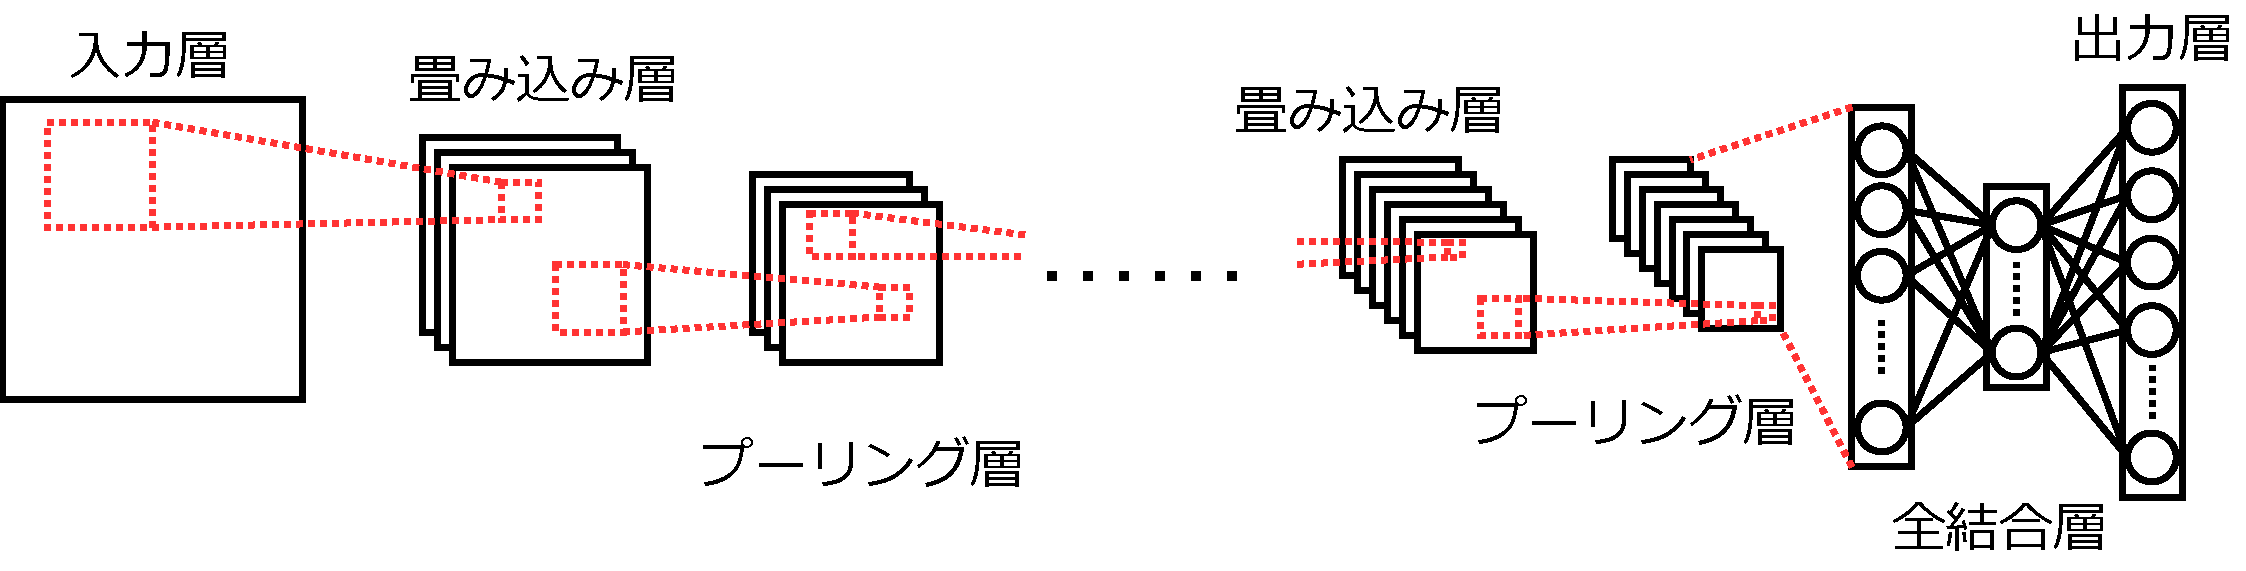
\includegraphics[scale=0.35]{./image/CNN_sample.pdf}
	\caption{CNNの概要}
	\label{fig:CNN_sample}
\end{figure}

図\ref{fig:CNN_sample}のようにCNNは畳み込み層とプーリング層と呼ばれる層が交互に重ねて構成され,全結合層へとつながる.
これらの層の概要を以下に示す.

\begin{itemize}	
	\item 畳み込み層
	
	畳み込み層は,データに対していくつかのカーネル(フィルター)を適用することで特徴を抽出する層である.
	カーネルは,事前に学習してデータ上に特徴を見つけた際に活性化させることができるようなカーネルを見つけて使用する.
	畳み込みによって得られた複数の特徴を特徴マップという.
	特徴マップの数は使用するカーネルの数に等しくなる.
	畳み込みの一例を図\ref{fig:conv_sample}に示す.
	ここでは,簡単のため入力データとカーネルの数値は0と1の2値とする.
	\begin{figure}[H]
		\centering
		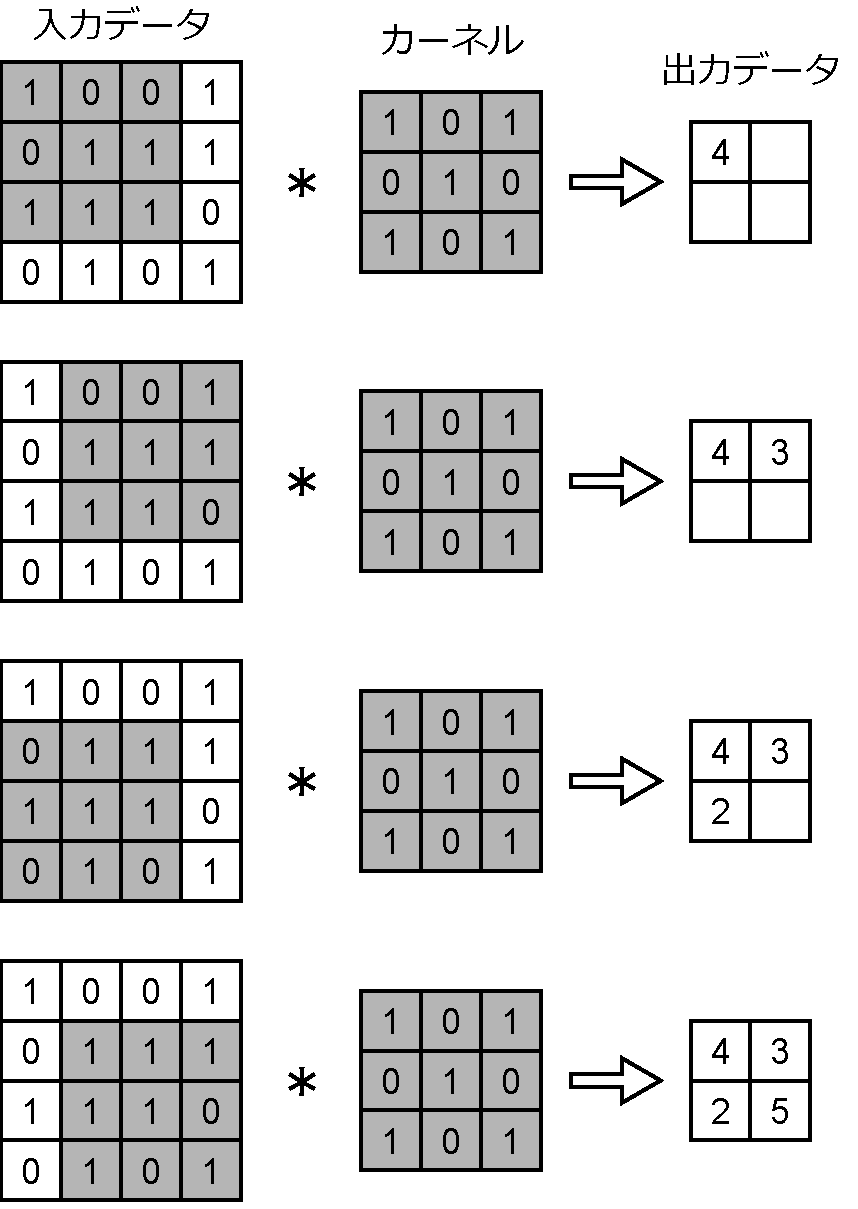
\includegraphics[scale=0.5]{./image/conv_sample.pdf}
		\caption{畳み込みの一例}
		\label{fig:conv_sample}
	\end{figure}
	
	
	
	\item プーリング層
	
	プーリング層は,データ量を減らす変換を行う層である.
	これにより,後に続く層の計算量を削減することができる.
	本研究では,近傍の入力値の最大値を出力するMAXプーリングを使用する.
	MAXプーリングの一例を図\ref{fig:pooling}に示す.
	\begin{figure}[H]
		\centering
		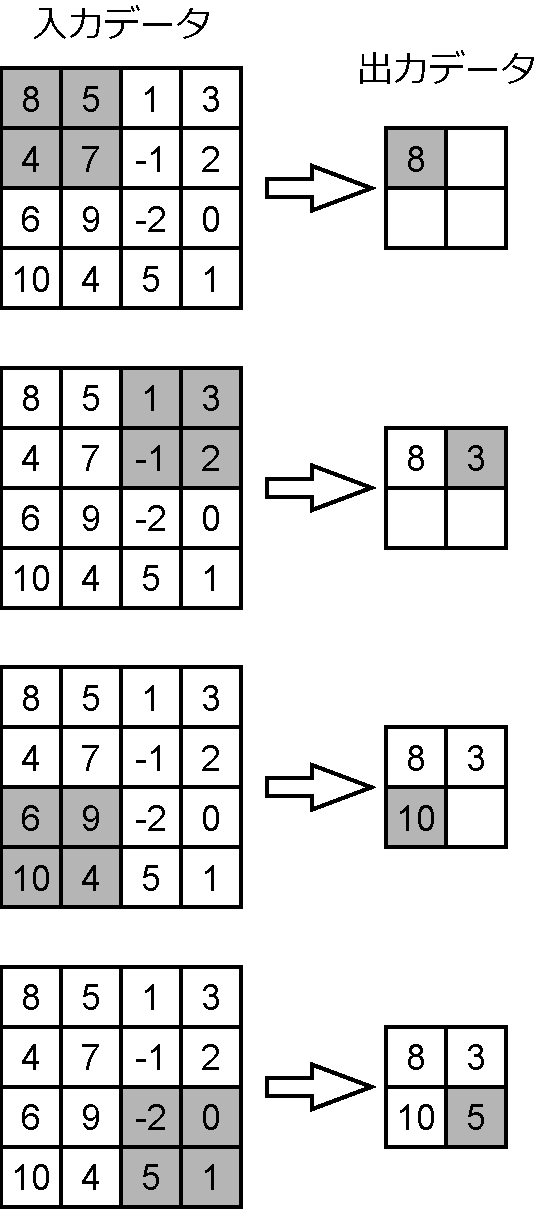
\includegraphics[scale=0.5]{./image/pooling.pdf}
		\caption{MAXプーリングの一例}
		\label{fig:pooling}
	\end{figure}
	
	\item 全結合層
	
	全結合層は,通常のニューラルネットワークと同様に重みとバイアスを用いて入力値を変換する層である.
	最後にソフトマックス関数を適用することで確率の表現に変換する.
\end{itemize}

通常のニューラルネットワークでは全てのニューロンが完全に結合しているため,少しだけずれたわずかに違うデータでもまったく別のデータとして学習してしまい
柔軟性や汎化能力に欠けるが,CNNではニューロン同士の結合はカーネルの大きさに制限されるため,わずかに違うデータにも対応できるといった利点がある.


\section{結言}

本章ではソフトウェアメトリクスについて概説した.
ソフトウェアメトリクスにより......が可能である.
そこで次章では○○に基づいた△△を提案していく.

\chapter{○○に基づいた△△}
\label{chap:提案法}

\section{諸言}

\section{データの前処理}
本節ではデータの前処理に使用する抽象構文木とそれを実装するために用いたライブラリであるJavaParserについて説明する.

\subsection{抽象構文木}
抽象構文木(Abstract Syntax Tree : AST)とは,ソースコードの文法構造を木構造で表したものである.


ASTには,ファイル全体を表すルートノードがあり,その子としてノードが複数接続されている.
例えば,import文やクラスの宣言などが挙げられる.
そして,さらにクラスの宣言はフィールドやメソッドを表すノードに接続されている.
ASTの概要を図\ref{fig:抽象構文木}に示す.
図\ref{fig:抽象構文木}のルートノードに当たるCompilationUnitは,構築されたASTを受け取るクラスである.



\begin{figure}[H]
	\centering
	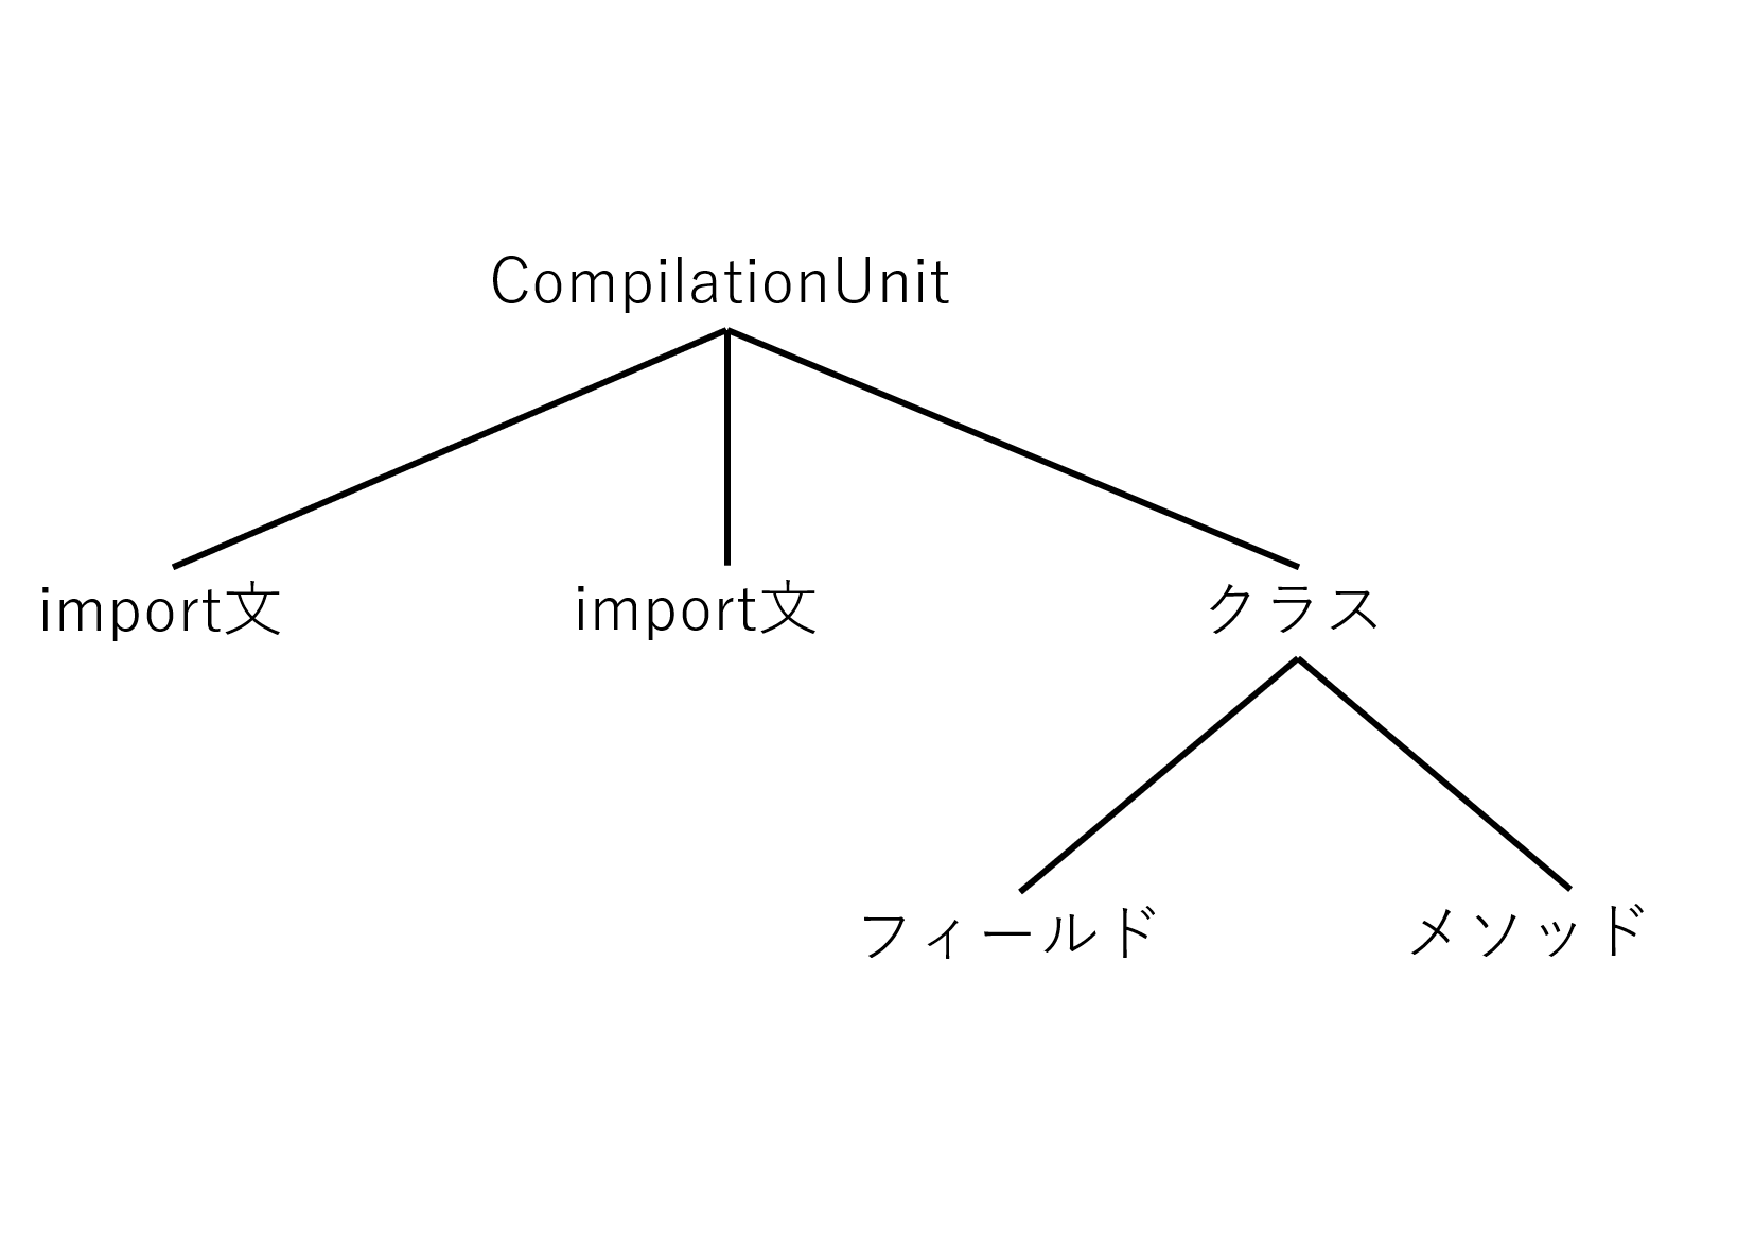
\includegraphics[scale=0.34]{./image/ast_image.pdf}
	\caption{ASTの概要}
	\label{fig:抽象構文木}
\end{figure}


ASTを利用することで,元の字句だけでなく,その字句の意味も同時に取得できる.
例えば,``int a;''という命令はaがint型の変数,intがPrimitiveTypeという意味を持ち,それを取得することができる.


\subsection{JavaParser}
Java言語で書かれたソースコードを解析し,そのASTを得るためにJavaParser\cite{JavaParser}というライブラリを用いる.
これにより,メソッドをトークン化したものを容易に取得できる.
JavaParserを使用して図\ref{sample}に示すSample.javaを解析したときの出力結果を図\ref{token_analy}に示す.
本研究では空白,改行,区切り文字は使用しないため,無視している.

\begin{lstlisting}[caption=Sample.java,label=sample]
public class Sample {
	public void main(String[] arg){
		for (int i = 0; i<10; i++) {
			System.out.println(i);
		}
	}
}
\end{lstlisting}


\begin{lstlisting}[caption=出力結果,label=token_analy]
public
class
sample
public
void
main
String
arg
for
int
i
=
0
i
<
10
i
++
System
out
println
i
\end{lstlisting}
図\ref{token_analy}のように意味のある文字列だけを取得し,ソースコードをトークン化することができる.
トークンを取得した後,forならForStatement,intならPrimitiveTypeといった,それぞれのトークンの意味を追加する.


この処理をメソッドの本体に対して行うことで,本研究に用いるデータセットを作成する.


\chapter{実験}
\label{chap:実験}

表 \ref{tbl:表の例} に表の例を示す.
\section{定義}

一般に,定義 \ref{def:距離} における(\ref{eqn:距離})式の関数 $d$ は
距離関数と呼ばれる\footnote{信じないでね.}.
距離関数が定義された空間{\--}正確にいえばベクトル空間{\--}を距離空間とい
う\footnote{これまた,信じないでね}.

\begin{definition}[距離] \label{def:距離} ~
	
	\begin{rm}
		$2$ つのベクトル $\boldsymbol{x}$, $\boldsymbol{y}$ が与えられたとき,
		これらの距離 $d(\boldsymbol{x},\boldsymbol{y})$ を次式で定義する:
		%
		\begin{equation}\label{eqn:距離}
			d(\boldsymbol{x},\boldsymbol{y}) = %
			|| \boldsymbol{x} - \boldsymbol{y} ||
		\end{equation}
	\end{rm}
	%
	\QED
\end{definition}

上の例のように定義や定理の終わり,
箇条書きの終わりに
\verb|\QED| と書くと,右寄せで □ が表示される.
数学では ``証明終わり'' の意味で使われるが,
工学の論文ではそれ以外でも一つの区切りであることを明記するために使うことがある.



\begin{table}[H]
 \centering
 \caption{簡単な表の例です}
 \label{tbl:表の例}
 \begin{tabular}{lcr} \Hline
  左寄せ & 中央揃え & 右寄せ \\ \Hline
  $1$ & JabRef\cite{JabRef} & $1.50$ \\ \hline
  $2$ & XYZ & $3.91$ \\ \hline
  $3$ & ZZZ & $1.83$ \\ \Hline
 \end{tabular}
\end{table}

多くの学術論文では表がよく使われるが,その際には縦の罫線を極力使用しない傾向にある.
特に両端の縦罫線は省略されることが多い.
学会によっては横罫線も可能な限り省略することが推奨される.

なお,(これも学会によるが,)横罫線の一部を太くするように指示されることがある.
本サンプルでは表の始まりと終わり,並びに項目名の下については太くしてある.
太くする場合は \verb|\hline| の代わりに \verb|\Hline| を使う.


\chapter{結論}
\label{chap:結論}

ダブルクォーテーションは ``このように'' 書く.

特殊記号は $\alpha$ という感じで前後に半角スペースを入れて書くことを推奨する.


\acknowledgement

例年の卒論を真似してお礼を書く.

\bibliographystyle{tipsj}
\bibliography{mybiblist}

\appendix

\chapter{その他}

ここでは番号がすべてアルファベットに変わる.

\end{document}


